\documentclass[letterpaper,10pt]{article}

\usepackage{titling}
\usepackage{listings}
\usepackage{url}
\usepackage{setspace}
\usepackage{subfig}
\usepackage{sectsty}
\usepackage{pdfpages}
\usepackage{colortbl}
\usepackage{multirow}
\usepackage{relsize}
\usepackage{amsmath}
\usepackage{fancyvrb}
\usepackage{amsmath,amssymb,amsthm,graphicx,xspace}
\usepackage[titlenotnumbered,noend,noline]{algorithm2e}
\usepackage[compact]{titlesec}
\usepackage[default]{droidserif}
\usepackage[T1]{fontenc}
\usepackage{tikz}
\usetikzlibrary{arrows,automata,shapes,trees,matrix,chains,scopes,positioning,calc}
\tikzstyle{block} = [rectangle, draw, fill=blue!20, 
    text width=2.5em, text centered, rounded corners, minimum height=2em]
\tikzstyle{bw} = [rectangle, draw, fill=blue!20, 
    text width=4em, text centered, rounded corners, minimum height=2em]

\definecolor{namerow}{cmyk}{.40,.40,.40,.40}
\definecolor{namecol}{cmyk}{.40,.40,.40,.40}

\let\LaTeXtitle\title
\renewcommand{\title}[1]{\LaTeXtitle{\textsf{#1}}}


\newcommand{\handout}[5]{
  \noindent
  \begin{center}
  \framebox{
    \vbox{
      \hbox to 5.78in { {\bf ECE155: Engineering Design with Embedded Systems } \hfill #2 }
      \vspace{4mm}
      \hbox to 5.78in { {\Large \hfill #4  \hfill} }
      \vspace{2mm}
      \hbox to 5.78in { {\em #3 \hfill} }
    }
  }
  \end{center}
  \vspace*{4mm}
}

\newcommand{\lecture}[3]{\handout{#1}{#2}{#3}{Lecture #1}}
\newcommand{\tuple}[1]{\ensuremath{\left\langle #1 \right\rangle}\xspace}

\addtolength{\oddsidemargin}{-1.000in}
\addtolength{\evensidemargin}{-0.500in}
\addtolength{\textwidth}{2.0in}
\addtolength{\topmargin}{-1.000in}
\addtolength{\textheight}{1.75in}
\addtolength{\parskip}{\baselineskip}
\setlength{\parindent}{0in}
\renewcommand{\baselinestretch}{1.5}
\newcommand{\term}{Spring 2014}

\singlespace


\begin{document}

\lecture{ 24 --- Software Lifecycle Models \& Tactics}{\term}{Jeff Zarnett, based on original by Patrick Lam}

\section*{Software Development Lifecycle}
If you're asked to develop a software project, you're likely to follow
a process that looks like this:

\begin{center}
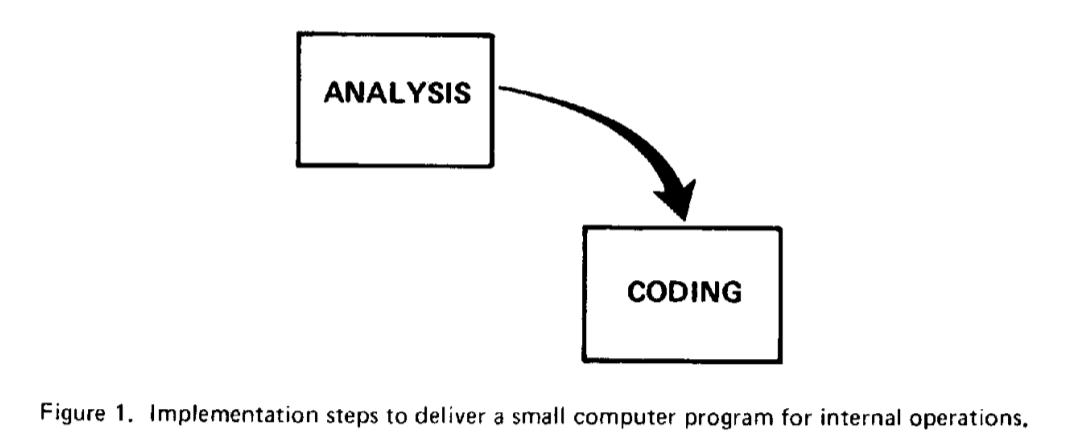
\includegraphics[width=.5\textwidth]{images/two-stages.png}
\end{center}

\noindent
(Figures are from~\cite{royce70:_manag_devel_large_softw_system}.)

This is fine, but it doesn't scale. You will fail if you try this on a
sufficiently-large project, or you will evolve some sort of more
refined process: managing large software projects is notoriously
difficult.  Software development lifecycles attempt to provide more
structure to keep the activities surrounding software development
on-track.

\paragraph{Death Marches.} Software projects in the industry are usually under some pressure: schedule pressure, budget pressure, and staff pressure. A little pressure is normal, but when a project is under so much pressure that the resources available for completion are so hopelessly inadequate there is no possibility of success, it is known as a \textit{Death March}. Some possible reasons for a project becoming a death march are: naive optimism, organizational politics, trying to build a huge project all at once, or just managerial incompetence \cite{DeathMarch}.

It is obvious we would like to avoid death marches, but how?

\paragraph{Key idea: Iterations.} Lifecycles always involve iterations of design
stages. More complex projects will typically have both more design stages
and more iterations. Lifecycle models help organize the stages of the design and implementation
process.

\paragraph{Process.} Good process can help with avoiding fiascoes and
death marches. Project management is a huge part of the software
development lifecycle. Without effective project management (of some
sort), a software project is likely to be delayed and poorly-designed.

The software design process resembles the engineering design process,
in that both attempt to build the best possible design given sets of
project requirements, project constraints, and criteria for evaluating
design success. We'll be talking about engineering design soon.

A key difference between general engineering design and software design is that
you can deploy software immediately after implementing it; 
typically, the result of engineering design gets dispatched to manufacturing
(or construction companies).

\subsection*{High-Level Overview}
A general list of steps in the software design
process is:

\begin{itemize}
\item Problem Definition
\item Requirements Development
\item Project Planning
\item High-Level Design
\item Detailed Design
\item Coding and Debugging
\item Integration Testing
\item System Testing
\item Corrective Maintenance
\end{itemize}

The different lifecycle models link these steps in various ways. If you follow a model, then good things may happen. Following a model poorly is a potential recipe for disaster, in the form of poorly designed
and implemented software, and many bug-fixing design iterations.


\subsection*{Waterfall Model}
The old classic idealized ``model of a software engineering process''
is the waterfall model.

\begin{center}
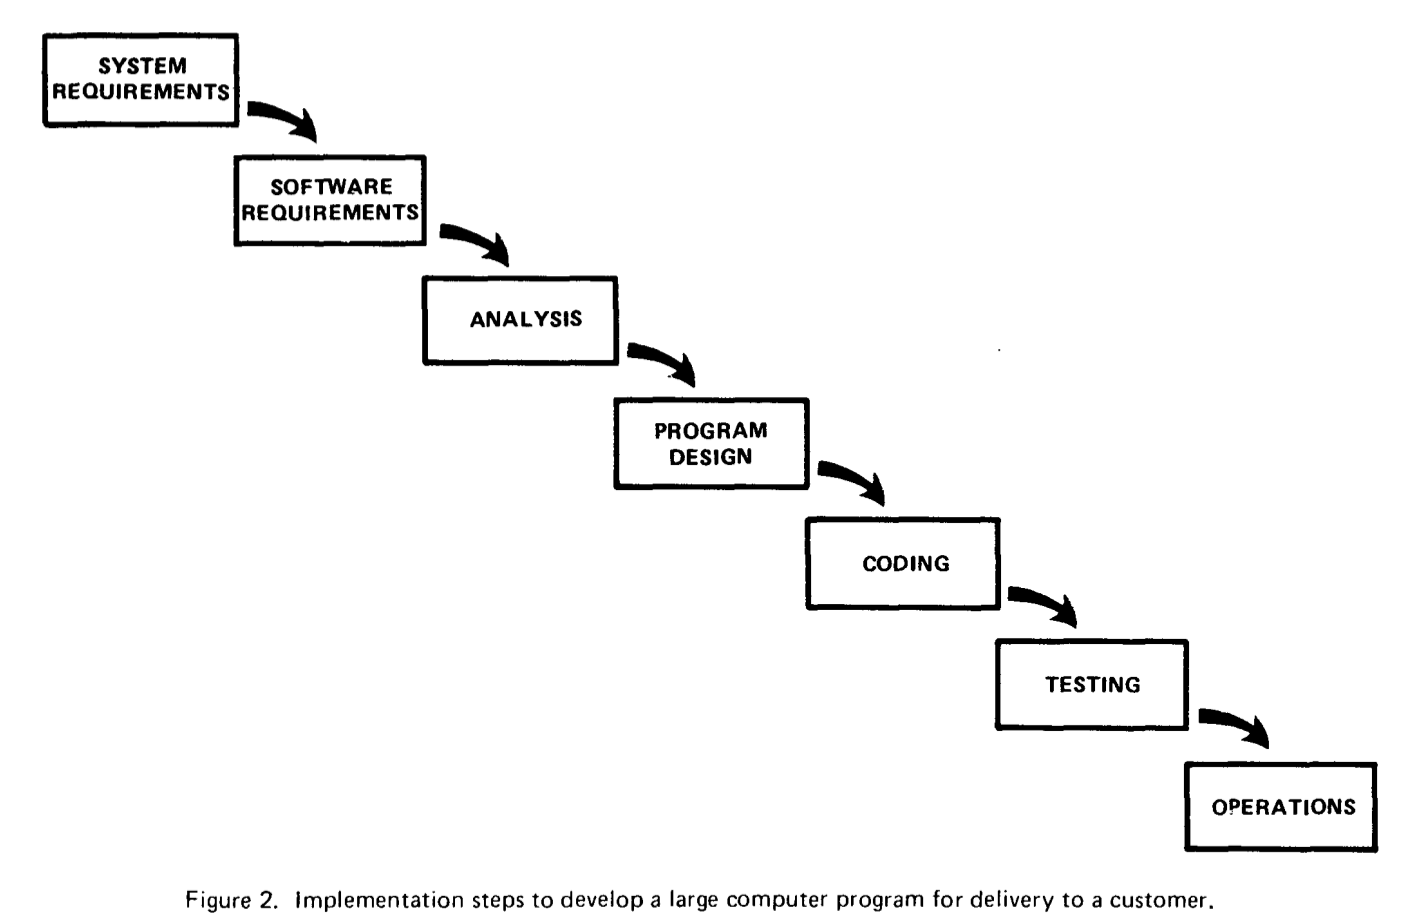
\includegraphics[width=.6\textwidth]{images/classic-waterfall.png}
\end{center}

\begin{itemize}
\item The waterfall model is highly sequential: stages may not overlap.
The project moves onto the next stage following a review.
\item Advantages: 1) it fixes customer requirements early in the design
process (hopefully the right requirements); 2) in principle, models like this
would identify
problems early in the design process, when changes are less expensive.
\item Disadvantages: 1) you're working blind, so that you don't see any
software until the end of the implementation stage (causing critical failures
in practice); and 2)
changes late in project development imply lots of wasted work.
\end{itemize}

{\bf Actually, no one seriously advocates this model---that is, it's a
straw man.}  Even in the original paper showing the waterfall model,
the author pointed out that you'd be more likely to get this:

\begin{center}
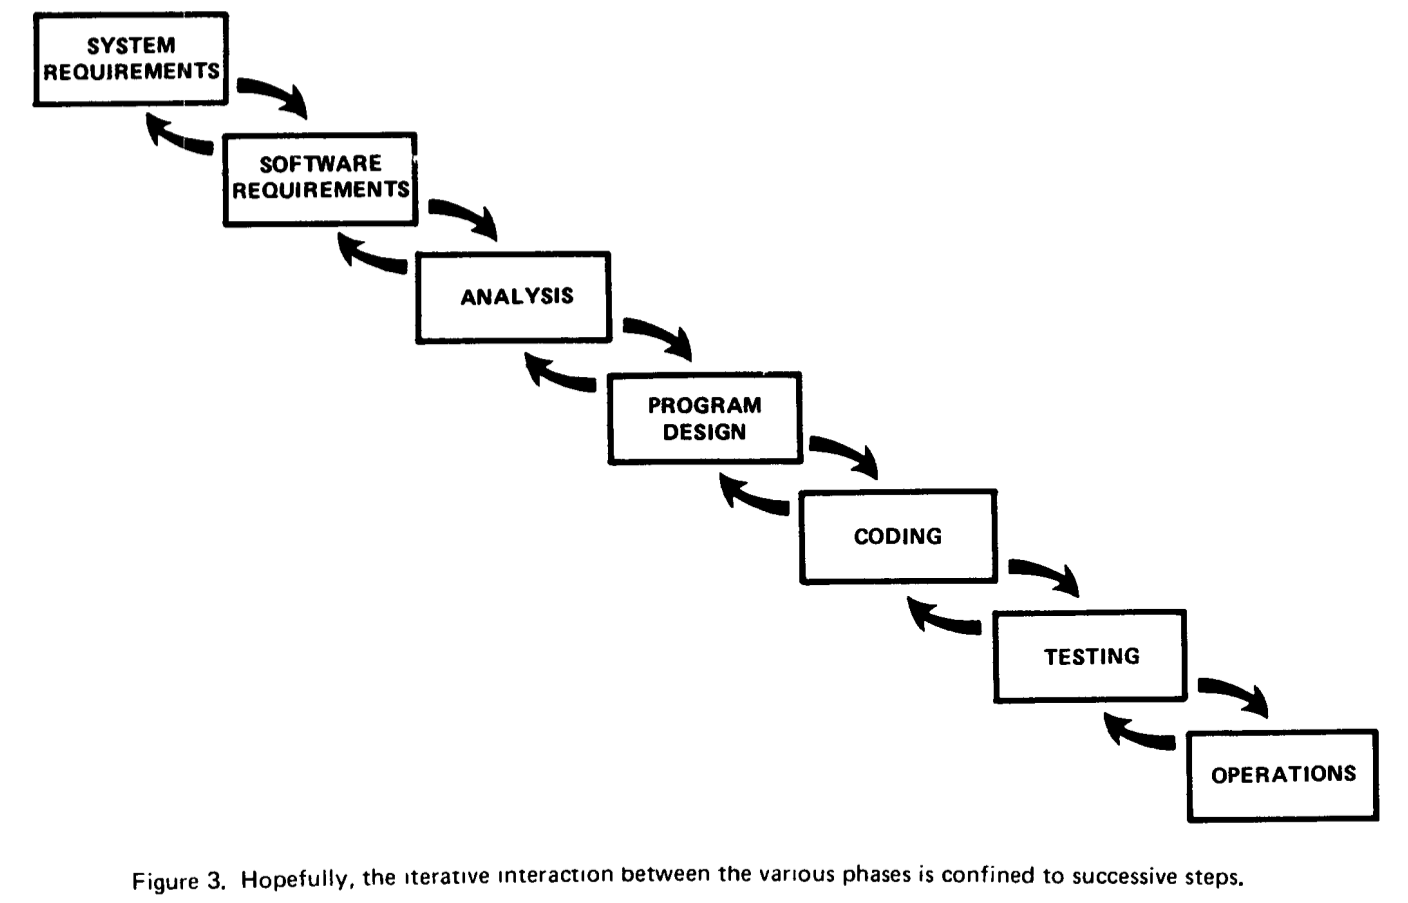
\includegraphics[width=.6\textwidth]{images/more-ideal-iteration}
\end{center}
and if you were less lucky, you'd get something more like this:
\begin{center}
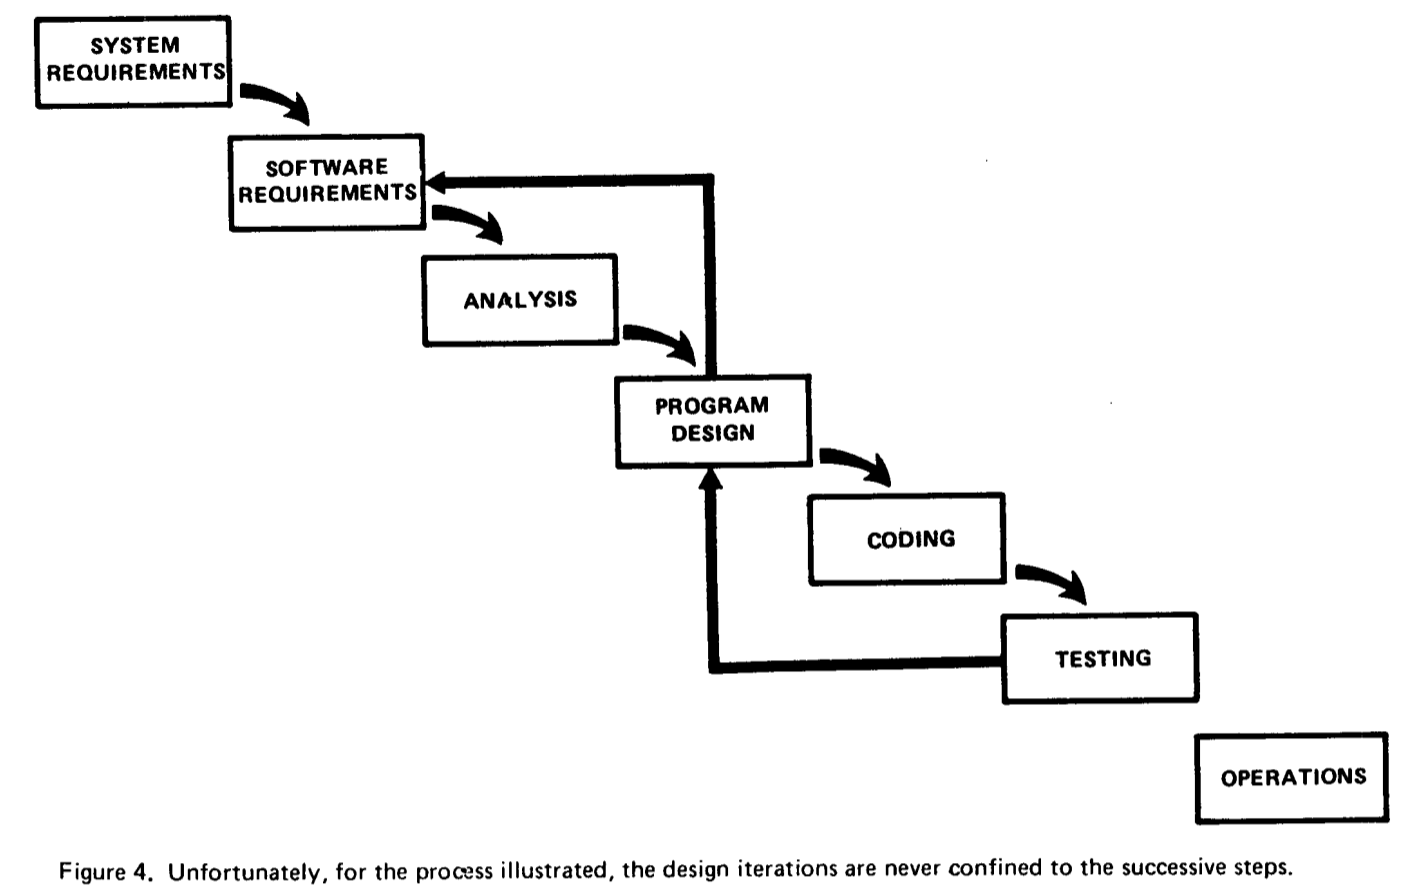
\includegraphics[width=.6\textwidth]{images/less-ideal-iteration}
\end{center}

\subsection*{Concurrent Engineering}
A variant on the waterfall model is the concurrent engineering model.
Instead of waiting on the previous stage to finish, you can start the
next stage once you have something to work with. Because the stages
overlap, this model is also known as the ``sashimi'' model.

\begin{center}
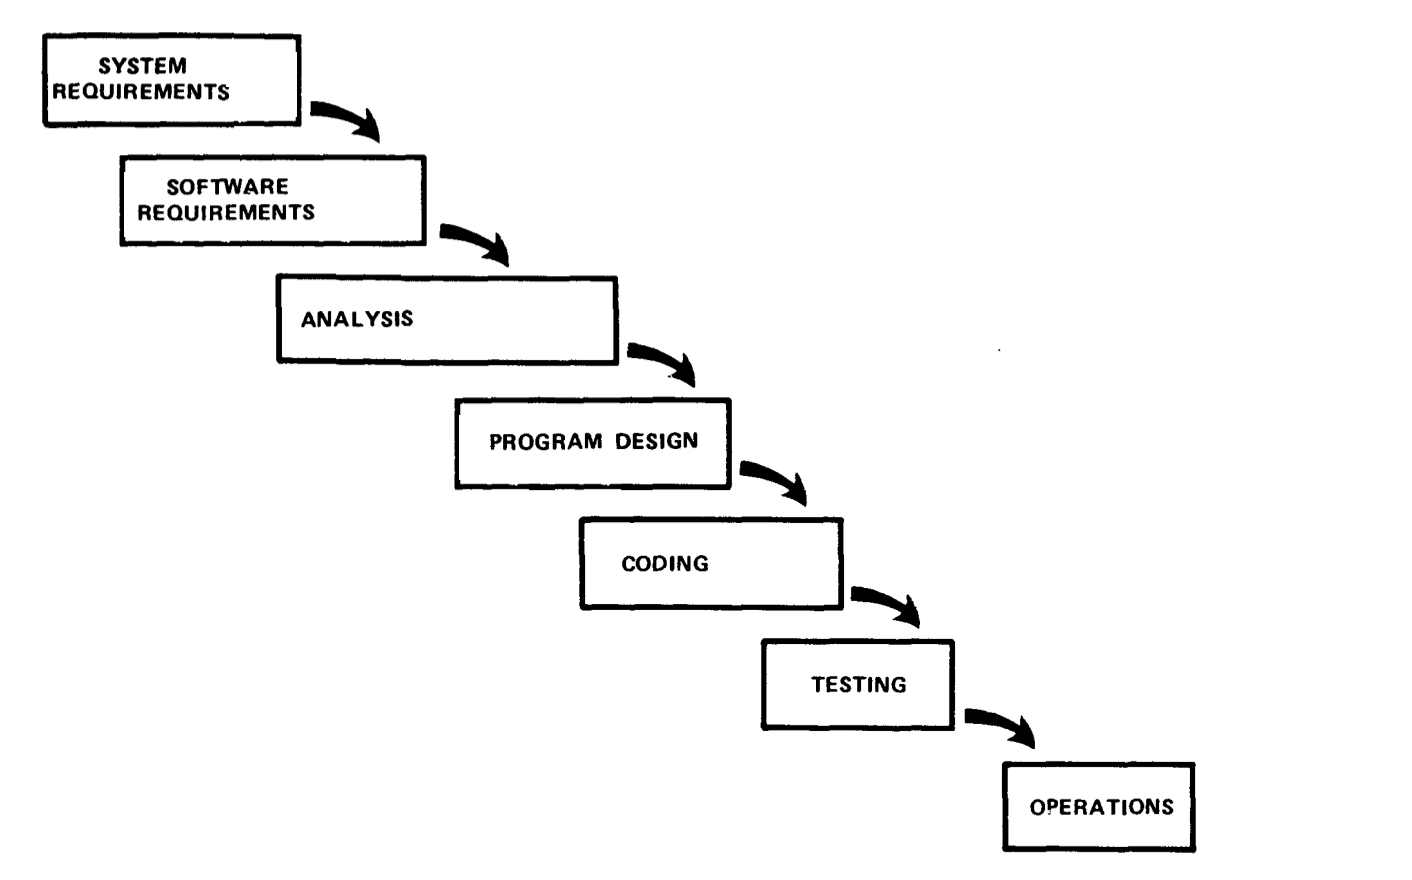
\includegraphics[width=.6\textwidth]{images/concurrent-engineering}
\end{center}

\begin{itemize}
\item The concurrent engineering model works well for many projects (why wait?)
Because you're trying to use the result of a stage, you are more likely to
discover problems with it and correct it, in collaboration with the team
that produced the result.
\item Advantages: 1) because you don't need to write down every last
  (irrelevant) detail, you might need less documentation; 2) projects need
  not be subdivided into smaller projects; 3) testing may reveal problems
  earlier in the development process.
\item Disadvantages: 1) milestones may be more ambiguous; 2) progress
  is difficult to track: how done is stage $x$?; 3) poor
  communication can lead to disaster in the presence of parallel design
  stages.
\end{itemize}


\subsection*{V-Model}
The V-Model is another variant of the waterfall model. Looking at the image, it is obvious why it is called the V-model. The goal is to make links between the early and late stage. For example, system verification and validation should correspond to the requirements and architecture. Although there are some additional links between the stages of the V-model, in practice, it is very similar to Waterfall and shares all the positives and negatives of Waterfall.

\begin{center}
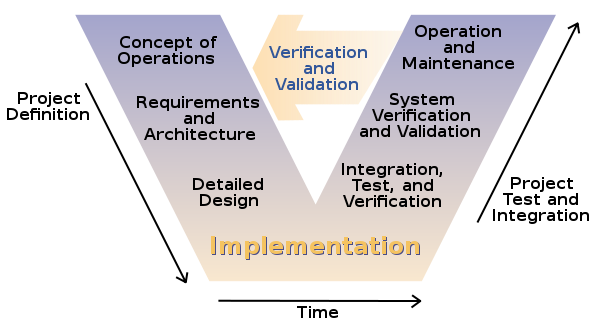
\includegraphics[width=.5\textwidth]{images/vmodel.png}
\hfill \url{http://en.wikipedia.org/wiki/File:Systems_Engineering_Process_II.svg}
\end{center}

\subsection*{Spiral Model}
The spiral model is a much more iterative process. 
You continue going through stages, in order, until you get to
a satisfactory solution. Projects are split into a number of smaller
sub-projects, with each iteration corresponding to a smaller project.
You'll iterate many times. Not all stages of the design process
require equal effort: testing may, and often does, require more effort
than coding.

\begin{center}
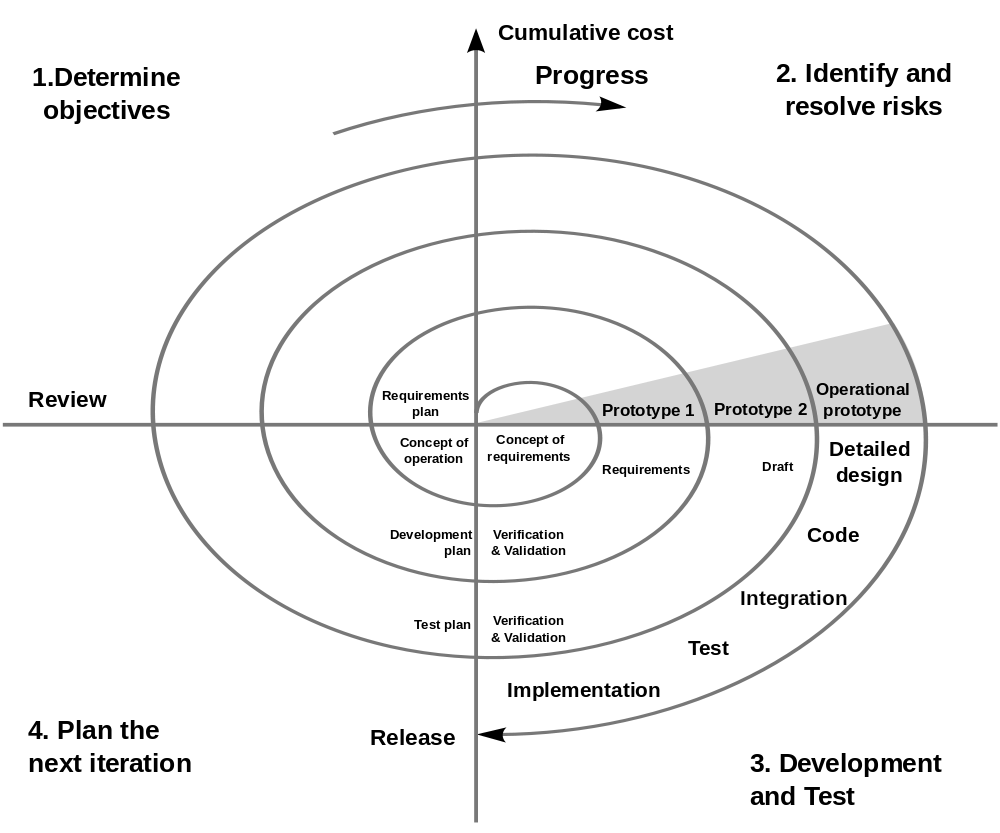
\includegraphics[width=0.75\textwidth]{images/spiral-boehm.png}
\hfill \url{http://en.wikipedia.org/wiki/File:Spiral_model_%28Boehm,_1988%29.svg}
\end{center}

\begin{itemize}
\item The spiral model is risk-oriented, and each sub-project addresses
one or more risks, in order of magnitude, until you get to a satisfactory
solution where all of the major risks
have been addressed. (We'll talk more about risks later).
\item Advantages: 1) this model addresses the biggest risks first, when
changes are least expensive; 2) progress is visible to the customer and
to management.
\item Disadvantage: some projects don't have clearly identifiable
sub-projects with verifiable milestones; this model is generally
identified with more heavyweight process than extreme programming.
\end{itemize}

\subsection*{Summary}
We've seen a lot of variants of the Waterfall model, but it's pretty well accepted in industry that the Waterfall model (and its variants) are considered obsolete if not outright harmful. Iterations are the accepted method for software development, and we'll look, in the next part, at iterations in detail.

\section*{Software Development Tactics}

We will now examine some lower-level tactics for software development.

\subsection*{Strawman: Cowboy Coding}
If there is no project management methodology in use (whether formal or informal), it is sometimes referred to as \textit{Cowboy Coding}. Cowboy coding is held up by some methodologies as what always happens without the use of their specific methodology, but it is only one possibility. In this ``model'', every developer just does whatever they want to do whenever they choose to do it. There are no design documents, no formal start or end to an iteration, and rarely any goals for what to have in an iteration. This might work on a hobby project done by 1-2 developers in their spare time, but it is unrealistic for use on commercial software projects. Nobody advocates this model, but it is worth mentioning.

\subsection*{Scrum}
In the Scrum development model, work is broken down into a series of ``Sprints'', which are short cycles of a specified length (such as 30 days). At the beginning of a sprint, the development team reviews the items in the backlog and sets goals for the sprint.  After that, no new features will be accepted. During the sprint, there are daily meetings to make sure things are on track. At the end of the sprint, the team collects feedback for the next sprint. \cite{scrum}

\begin{center}
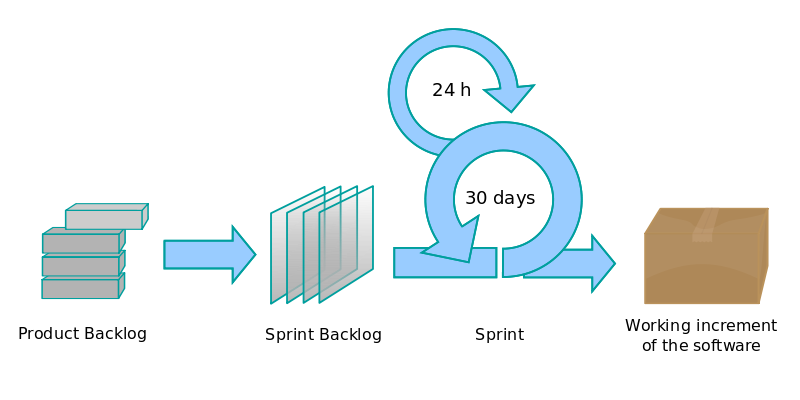
\includegraphics[width=0.7\textwidth]{images/scrum.png}
\hfill \url{http://en.wikipedia.org/wiki/File:Scrum_process.svg}
\end{center}

\begin{itemize}
	\item Advantages: 1) Short iterations mean lots of opportunities for input and feedback. 2) Daily meetings mean lots of co-ordination between team members. 3) It encourages breaking the software down into manageable units.
	\item Disadvantages: 1) It does not scale well to large teams. 2) Daily meetings can result in excessive overhead. 3) At the sprint deadline, development ends whether the code is finished or not, leading possibly to incomplete deliverables.
\end{itemize}

\subsection*{Test-Driven Development}
Normal behaviour in software development is that first the software is written and then the tests are created. Test-Driven Development (TDD) turns this around: write the tests first and then write the software. When a new feature is added, first the developer writes a test (and it should fail). Then the feature is developed until the new test passes. Then the process repeats until the feature is done. Then the developer refactors the code. More time is spent developing the unit tests, but it may save time in the long run. \cite{Beck}

We will talk about unit tests later on in the term. There is also a 4th year ECE class on Software Testing. Refactoring is also a subject we will cover later in ECE 155, but for now you can just take ``refactor'' to mean ``clean up''.

\begin{center}
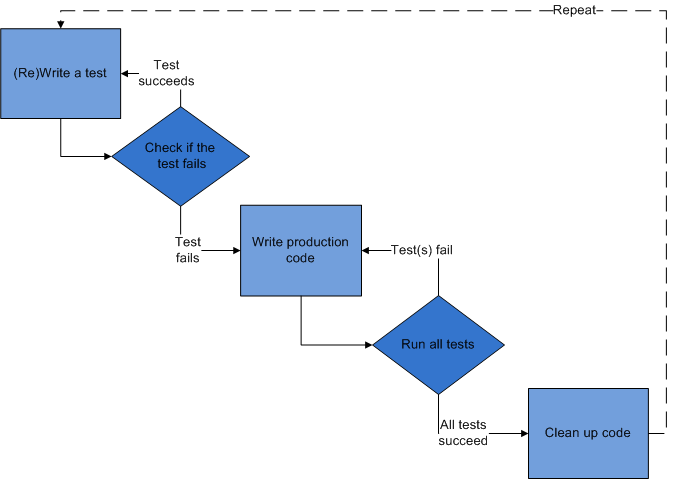
\includegraphics[width=0.7\textwidth]{images/tdd.png}
\hfill \url{http://en.wikipedia.org/wiki/File:Test-driven_development.PNG}
\end{center}

\begin{itemize}
	\item Advantages: 
		1) This model emphasizes testing in a way that other models do not. Unfortunately, when time is short and the product needs to be released, testing is one of the first things to be cut; in TDD, that does not happen. 
		2) More code will be covered by the tests.
		3) It encourages breaking the software down into testable units.
	\item Disadvantages:
		1) Unit tests are created by the same people who write the code, so an error in the code may be undetected because of a similar error in the unit test.
		2) Not everything is testable: database interactions, user interface, etc.
		3) TDD focuses only on unit tests, and this is not the only kind of testing.
		4) It's possible to create too many redundant tests, or inflexible tests that cannot be adapted when the software changes.
		5) When tests are broken there is a tendency to disable them or just implement a quick change to ``fix'' the test, without considering the meaning of the change.
		6) Passing tests are not the same thing as functioning, useful software.
\end{itemize}

\subsection*{Behaviour Driven Development}
Behaviour-Driven Development (BDD) is a modification of Test-Driven Development, combining the principles of TDD with Object-Oriented Programming. It was developed to answer several questions that arise out of TDD, such as where to start, how much to test at once, and what to name the test methods. In BDD, the tests are still written before the unit is implemented. Tests should be created in the order of business value: the most important things get tests written next. If the behaviour cannot be described in a single sentence, it means multiple tests are required. Each test gets a sentence as its name, such as \texttt{testFailsForDuplicateCustomers()}. The name is descriptive once you remove ``test'' and put spaces between the words: ``Fails For Duplicate Customers'' \cite{bdd}.

BDD also features \textit{Stories} which are a description of a requirement and benefit; we'll talk about those when we get to the lecture about software requirements \cite{bdd2}.


\subsection*{Extreme Programming}
We can call extreme programming~\cite{Beck:2004:EPE:1076267}, or XP, another
software lifecycle model, although it differs from the other models
quite a bit. It's closest to the spiral model, scaled down and made
more agile. The initial idea was to take the ``good'' parts of good
programming practice, like reviews and testing, and ``crank up all the knobs to
10''\cite{ivkb}
on those, leaving everything else behind.

\paragraph{Agile Methodologies.} XP is one of several agile methodologies,
which all attempt to be less bureaucratic than the traditional
``heavyweight'' methodologies. 

\paragraph{Values.} XP supports five values in software development:

\begin{itemize}
\item Communication:
 Work together. Includes pair programming. Face-to-face communication.
 Workspaces to support collaboration. Don't generate paperwork.
 Share knowledge.
\item Simplicity:
Don't do more than you need to. Take small, simple steps to goal.
``You Ain't Gonna Need It''. Requires refactoring later.
\item Feedback:
 Get feedback from system (unit tests), from client (functional/acceptance 
 tests), from the team (time estimates). Demo working software.
\item Courage:
 Code for today, not tomorrow.
 Refactor when necessary, don't be scared.
 Throw code away when necessary.
 Work together to avoid failure and don't fear it.
\item Respect:
 Respect contributions of other team members (devs and customers).
 Management must respect judgment of programmers.
 Don't break the build or otherwise waste others' time.
\end{itemize}

\subsection*{Activities} 
XP contains four basic activities: coding, testing, listening and
designing.

\paragraph{Coding.} The code is central to XP (versus requirements documents
or other specifications). XP attempts to get working code out as soon
as possible, even if the code has limited scope. Programmers pair up to
produce the code.

Besides its functional role, code also serves as a communication and 
experimentation medium.

\paragraph{Testing.} XP advocates test-driven development: before
and while implementing a feature, write down and implement automated
test cases (unit tests) for that feature. Run the test cases, ensure
that the feature doesn't work, then implement the simplest possible
thing that implements the feature. Code must always pass all of the
unit tests.

\paragraph{Listening.} As part of ensuring that the system does the
right thing, XP includes acceptance tests, which are created by the
on-site customer. These tests help ensure that the system does the
right thing.

More generally, the developers need to listen to the business side
of the organization about their areas of expertise, and vice-versa.

\paragraph{Designing.} XP does not advocate a big up-front design.
Instead, developers are supposed to create a design incrementally by
constantly re-factoring the code (more later) as it is written.

There are a number of practices which constitute extreme
programming, alluded to above.

\subsection*{XP Advantages}
XP can help avoid getting caught in bureaucratic tarpits. When you have 
a good team, XP should be able to deliver good results, creating simpler
designs that solve the appropriate problems, and responding well to changes
in requirements.

\subsection*{XP Disadvantages and Controversies}
Kent Beck says that XP works best when one uses all of the practices
together. Some of the practices can work alone, like test-driven
development. Others may not work as well in 
isolation\cite{srsn}. (``... ring of poisonous snakes, daisy-chained together.'') 
XP tends to work best with smaller-sized groups, i.e. less than a
dozen members.
The lack of up-front design and requirements specifications can be
worrisome.


\subsection*{Kanban}
Kanban is the Japanese word for ``visual card'', and its use started with the manufacturing process at the car company Toyota. Toyota does use physical cards, but in software development it could be a virtual card or a physical one on a board. It is meant to support non-centralized production control where work is ``pulled'' when the puller is ready, rather than ``pushed'' by someone else. In this system, the strategy is to prevent teams or developers from becoming overloaded; being overloaded results in waste, stress on the team members, or lower quality \cite{netobj}.

A key idea is to identify the ``bottleneck'' in the system: the stage of production that limits the rate of output. Imagine software as a pipeline with feature requests as the input and (working) software as the output. If developers can produce ten features per week but testers can test only five features per week, the testers are the limiting factor. Work that is done will pile up in front of the testers, who have a backlog, and in most cases the testers will start to catch up by cutting corners and skipping some testing, resulting in software with more bugs being shipped to the users \cite{kbb}.

Unlike Scrum or an iterative model, there are not necessarily defined iterations (sprints). The physical or virtual cards are represented on a board that is divided into different categories. A card represents a unit of work and it cannot proceed through the process (or pipeline) unless there is space farther along in the pipeline. 

\begin{center}
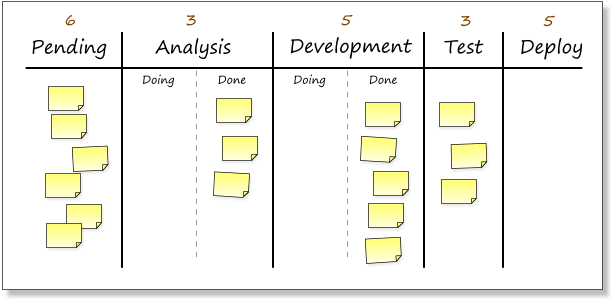
\includegraphics[width=0.7\textwidth]{images/kanban-board-1.png}
\hfill \url{http://www.kanbanblog.com/explained/image/kanban-board-1.png}
\end{center}

\begin{itemize} 
	\item Advantages: 1) Make bottlenecks visible; more visibility makes it easier to find and fix them. 2) Prevent overloading of one stage (and the problems that follow that). 3) Estimation is not present, so no time is spent on that; it all goes to implementation.
	\item Disadvantages: 1) A stoppage in one part of the process can stop many others; should developers just sit there with nothing to do because analysis is delayed? 2) Estimation might be important in a project. 3) No commitment - in other models a piece of work is promised in a certain iteration; Kanban views the process as continuous. 
\end{itemize}

\section*{Design and Planning}
We'll start by comparing design and planning for traditional engineering
projects versus software projects.
Traditionally, you would:\\[-2.5em]
\begin{itemize}
\item solicit requirements;
\item make a design;
\item analyze the design (with calculus);
\item stamp and sign the plan.
\end{itemize}~\\[-2.5em]
Then, someone else implements/builds the plan.

People tried this for software as well:\\[-2.5em]
\begin{itemize}
\item solicit requirements;
\item make UML diagrams; 
\end{itemize}~\\[-2.5em]
and hire code monkeys to implement the design.

\noindent However, this works poorly.

\paragraph{The Role of Prototyping.} Requirements are always difficult to 
formalize; this is a problem for all types of engineering, and
definitely for software. Prototyping is one way to mitigate the risk
of building the wrong thing.

\begin{quote}
The management question, therefore, is not {\em whether} to build a pilot system and throw it away. You {\em will} do that. [\ldots] Hence {\em plan to throw one away; you will, anyhow}.
\end{quote}
\hfill Frederick Brooks~\cite{mmm}.

The waterfall model is a straw-man for many reasons, but the
biggest one is because it pretends that prototypes aren't necessary.
You can never build a system without a prototype, because you never
really know what you need until you see it.  What's more, needs change
over time.

Another solution to the problem of shifting and unknown requirements,
along with prototypes, is the concept of \emph{iteration}. Different
models have different iteration strategies.

\paragraph{Agile Lifecycle Models.} The key point is to recognize
that change is inevitable, and to deal with it on-demand. Agile
models, such as extreme programming, advocate dealing with change
on-demand. In principle, they can handle changing requirements much
more smoothly.

However, agile models require suing developers, who must be good at
communicating with each other---these models are always highly
collaborative. Due to collaboration, agile methods are
supposedly resistant to 1) changes to the team over time and
2) differences between experience levels of the developers.

\subsection*{Choosing a Lifecycle Model}
Recall that the main difference between models is the pace of iteration.
\begin{itemize}
\item With large teams, diverse stakeholder groups: slower iterations;
\item With small teams, uncertain requirements, complex technologies: faster iterations.
\end{itemize}

\subsection*{Questions to Think About}
The answers to these questions will affect the pace of iteration and
hence the lifecycle model which you'll want to select.\\[-2em]
\begin{itemize}
\item Do you understand the customer requirements?
\item Will you need to make major architectural changes?
\item How reliable does the system need to be?
\item How much future expansion and growth do you foresee?
\item How risky is the project?
\item Is the schedule heavily-constrained?\footnote{Note: wishing for faster progress won't make it so.}
\item What is going to change during development?
\item How much do customers need visible progress?
\item How much does management need visible progress?
\item What experience does the design team bring?
\end{itemize}

\subsection*{Software Process Improvement}
One of the things you can
design is the design process itself. Here's what you can do to try to 
improve your software lifecycle model:\\[-2.5em]

\begin{itemize}
\item first, figure out what you mean to be doing: document your organization's software process;
\item next, figure out what you're actually doing: ensure that you're following the existing process; 
\item finally, identify areas of potential improvement and implement them.
\end{itemize}

In continuous process improvement, you constantly review the software
development process and its effect upon development. Continuous improvement 
also implies identifying and fixing issues that are
beyond the scope of individual projects: you can find and apply best
practices to all projects. Changes can allegedly yield dramatic
increases in development capability.



\bibliographystyle{alpha}
\bibliography{155}


\end{document}